% Appendix section: dataset-construction figure (promised to reviewer Fbco in the rebuttal:
% "We add a Background section ... and a dataset-construction figure").
% Appendix G. Integrated 2026-09-27 (third pass) from the verified draft
% scratchpad/neurips_promises/drafts/app_construction.tex; the figure is
% figs/fig_app_construction.pdf (TikZ source: drafts/fig_app_construction.tex). Bib entry
% Schwing2026CTSpinoPelvic1KArxiv is in bib/references.bib. Refers to app:release
% (appendix/release_split.tex) and sec:dataset (main text).
% Every number and its source: app_construction_NOTES.md.
\section{How the April 2026 release was built}
\label{app:construction}

Figure~\ref{fig:construction} traces the April 2026 release
(\S\ref{sec:dataset}) from its three sources to the records
the experiments used. It is adapted from the construction
figure of the dataset
article~\citep{Schwing2026CTSpinoPelvic1KArxiv}, which describes
the later v11 release; the steps only v11 has are left out
and are listed in Appendix~\ref{app:release}. The placement
step counts 804 patients, 352 of them separate and 90
spine-only. The orientation review excluded one separate
patient, and one placed spine-only patient is absent from
the export for a reason the export did not record, so the
release holds 351 separate and 89 spine-only patients.
A front-to-back mirror is not a rotation. In the two of the
nine checked, tokens 75 and 480, the released CT shows the
liver on the left. The six hip-label swaps match the labels
to the side of the image, which for 480 is the mirror of the
patient's; the other seven were not rendered.

\begin{figure}[ht]
\centering
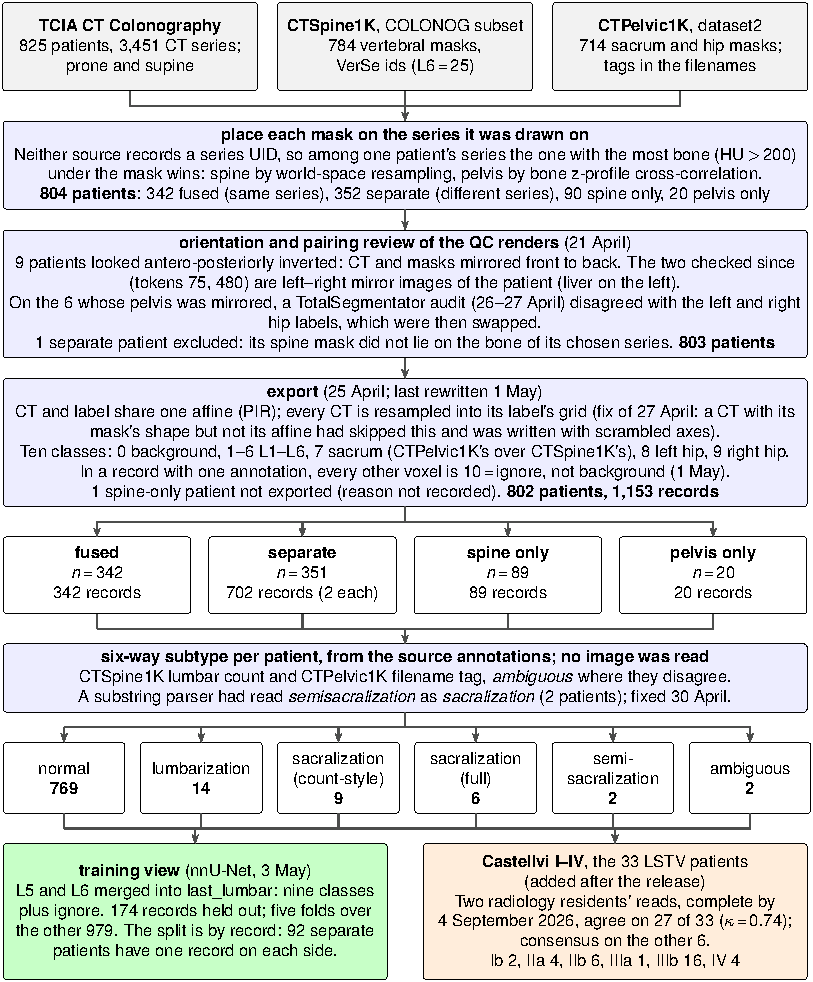
\includegraphics[width=\linewidth]{figs/fig_app_construction.pdf}
\caption{Construction of the April 2026 release of \dataset{},
on which every segmentation experiment here was run: 802
patients, 1{,}153 records; \textit{n} counts patients. Grey,
sources; blue, the April pipeline; green, the training view;
orange, added after the release. Adapted from Fig.~1 of the dataset
article~\citep{Schwing2026CTSpinoPelvic1KArxiv}, which describes a
later release (v11).}
\label{fig:construction}
\end{figure}
